\documentclass{beamer}

\usetheme{Boadilla}

%\includeonlyframes{current}

\usepackage{times}
\usefonttheme{structurebold}
\usepackage{listings}

\usepackage{pgf}
\usepackage{tikz}
\usepackage{alltt}
\usepackage[normalem]{ulem}
\usetikzlibrary{arrows}
\usetikzlibrary{automata}
\usetikzlibrary{shapes}
\usepackage{amsmath,amssymb}
\usepackage{rotating}
\usepackage{ulem}

%\setbeamercovered{dynamic}
\setbeamertemplate{footline}[page number]{}
\setbeamertemplate{navigation symbols}{}
\usefonttheme{structurebold}

\title{Software Testing, Quality Assurance \& Maintenance---Lecture 1}
\author{Patrick Lam\\University of Waterloo}
\date{January 4, 2017}

\colorlet{redshaded}{red!25!bg}
\colorlet{shaded}{black!25!bg}
\colorlet{shadedshaded}{black!10!bg}
\colorlet{blackshaded}{black!40!bg}

\colorlet{darkred}{red!80!black}
\colorlet{darkblue}{blue!80!black}
\colorlet{darkgreen}{green!80!black}

\newcommand{\rot}[1]{\rotatebox{90}{\mbox{#1}}}
\newcommand{\gray}[1]{\mbox{#1}}

\newenvironment{changemargin}[1]{% 
  \begin{list}{}{% 
    \setlength{\topsep}{0pt}% 
    \setlength{\leftmargin}{#1}% 
    \setlength{\rightmargin}{1em}
    \setlength{\listparindent}{\parindent}% 
    \setlength{\itemindent}{\parindent}% 
    \setlength{\parsep}{\parskip}% 
  }% 
  \item[]}{\end{list}}

\begin{document}

\begin{frame}
  \titlepage
\end{frame}

\begin{frame}
  \begin{center}
  \Huge ``The Testing Course''
  \end{center}
\end{frame}

\begin{frame}
\frametitle{Course mechanics}

\Large

\begin{changemargin}{1em}
  Office Hours: M 12:30-13:30, DC2597C\\[1em]
  
  Textbook: none\\[1em]

{\small
  \begin{tabbing}
Website~~ \= \url{http://patricklam.ca/stqam}\\[1em]
Github \> \url{git@github.com:patricklam/stqam-2017.git}\\[1em]
Piazza \> (you know where to find it)
  \end{tabbing}
}

  Grace days: You may submit assignments \\ up to 2 days late in total.
\end{changemargin}

\end{frame}

\begin{frame}
  \frametitle{Evaluation}
  \Large
\begin{changemargin}{1em}
\begin{tabular}{lr}
3 individual assignments & 20\% \\
& ~~(6 2/3\% each) \\
Course project (up to 3/group) & 15\% \\
Midterm & 15\% \\
Final exam & 50\% \\
\end{tabular}~\\[1em]

Midterm, final are open-book, open-notes.\\[1em]

\end{changemargin}

\end{frame}

\begin{frame}
  \frametitle{Failures}

\Large
\begin{changemargin}{2em}
  Let's consider:

\begin{itemize}
\item consequences;
\item causes; 
\item avoidance (before it's too late); 
\begin{itemize}
\item \Large testing
\end{itemize}
\item mitigation (afterwards).
\end{itemize}
\end{changemargin}
\end{frame}


{ % all template changes are local to this group.
    \setbeamertemplate{navigation symbols}{}
    \begin{frame}[plain]
        \begin{tikzpicture}[remember picture,overlay]
            \node[at=(current page.center)] {
                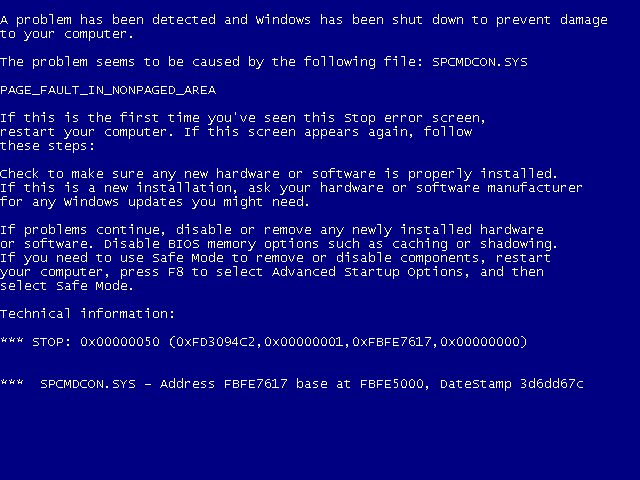
\includegraphics[width=\paperwidth]{L01/Windows_XP_BSOD.png}
            };
        \end{tikzpicture}
     \end{frame}
}
\begin{frame}
  \frametitle{Some Failures}
  %\framesubtitle{http://www.epicfail.com/wp-content/uploads/2010/01/vending-machine-fail.jpg}

%http://www.epicfail.com/wp-content/uploads/2010/01/vending-machine-fail.jpg

  \Large
  \begin{changemargin}{2em}

\begin{center}

\includegraphics[height=.5\textheight]{L01/vending-machine-fail.jpg}~~
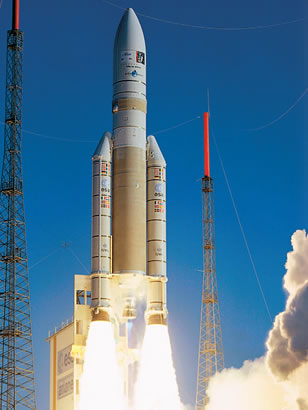
\includegraphics[height=.5\textheight]{L01/s2_2sm.jpg}
\end{center}

Who suffers from failures?
  \end{changemargin}

% end users
% in the case of Microsoft, framework providers suffer reputation harm

{\tiny Photos: (L) epicfail.com; (R) copyright ESA/CNES/ARIANESPACE - Service Optique CSG}

\end{frame}

\begin{frame}
  \frametitle{More Failures}

%http://www.microsoft.com/presspass/images/gallery/logos/web/mslogo-1.jpg

%% \begin{center}
%% 
\includegraphics[height=1em]{L01/mslogo-1.jpg}
%% \end{center}

% http://hermosodia.wordpress.com/2008/10/19/definicion-visual-de-workaround/
% http://hermosodia.files.wordpress.com/2008/10/workaround.jpg

\begin{center}

\includegraphics[height=4em]{L01/workaround.jpg}\\
\tiny \tt http://hermosodia.wordpress.com/2008/10/19/definicion-visual-de-workaround/
\end{center}

% http://www.cdc.gov/niosh/face/stateface/mi/04mi074.html

\begin{center}
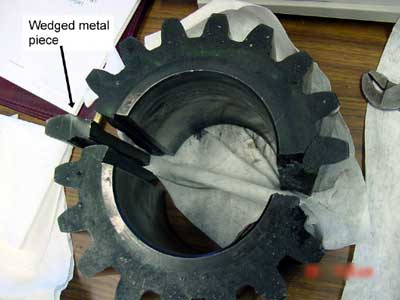
\includegraphics[height=4em]{L01/04MI074c.jpg}\\
\tiny (United States Centre for Disease Control, 04MI074)
\end{center}

% http://www.flickr.com/photos/stepman/2873443918/
\begin{center}
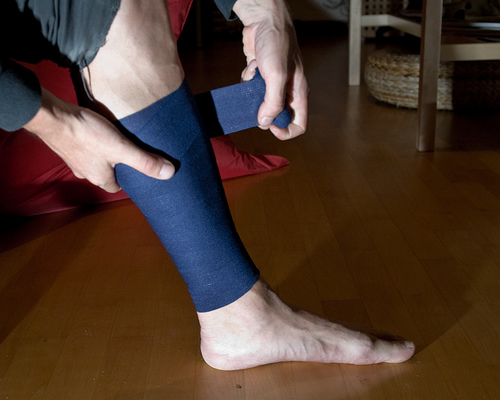
\includegraphics[height=4em]{L01/2873443918_ddc0337d19.jpg}\\
\tiny (stephen mantler at Flickr, ``A runner's injury'')
\end{center}

\end{frame}


\begin{frame}
  \frametitle{Infamous Software Bugs}
  \Large
  \begin{changemargin}{2em}
    Therac-25, 1985--1987: \\
    \qquad 5 deaths, severe injuries\\
    \qquad race conditions, no automated testing\\[1em]
    Northeast blackout, 2003\\
    \qquad (no ice storm)\\[1em]
    Ariane 5 crash, 1996\\[1em]
    Morris Worm, 1988
    
  \end{changemargin}
\end{frame}


\begin{frame}

  \frametitle{Why Does Software Go Wrong?}

\begin{center}
  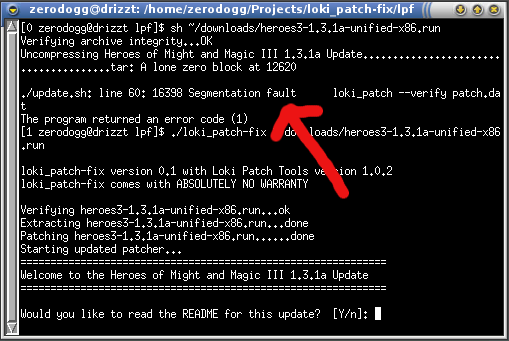
\includegraphics[height=0.6\textheight]{L01/lpf.png}
\end{center}

\begin{changemargin}{2em}
  1. Segfaults---or crashes; infinite loops too.
\end{changemargin}

\end{frame}

\begin{frame}

  \frametitle{Why Does Software Go Wrong?}

\begin{changemargin}{2em}
\begin{alltt}
    public int add(int x, int y) \{ \\
\qquad      return x - y; \\
\}

\end{alltt}
~\\[1em]
\Large
  2. Wrong Output:
\begin{itemize}
  \item method or module returns wrong information or has unwanted side effect.
\end{itemize}
\end{changemargin}

\end{frame}

\begin{frame}

  \frametitle{Why Does Software Go Wrong?}

  \begin{changemargin}{2em}
    3. Wrong API
\begin{itemize}
  \item a library can't do what you need it to do; or
  \item subsystems don't work together correctly.
\end{itemize}

\begin{center}
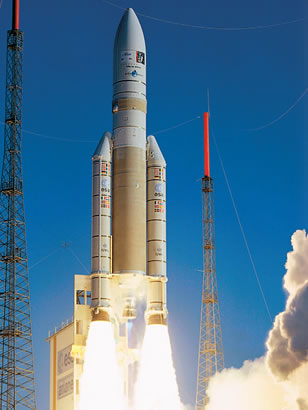
\includegraphics[height=.5\textheight]{L01/s2_2sm.jpg}
\end{center}

{\tiny Photo copyright ESA/CNES/ARIANESPACE - Service Optique CSG}
  \end{changemargin}
  
\end{frame}

\begin{frame}

  \frametitle{Why Does Software Go Wrong?}

  \begin{changemargin}{2em}
  4. Bad system-level behaviour:
\begin{itemize}
  \item Wrong output to user.
  \item Bad security.
  \item Wrong specifications.
\end{itemize}
  \end{changemargin}
\begin{center}
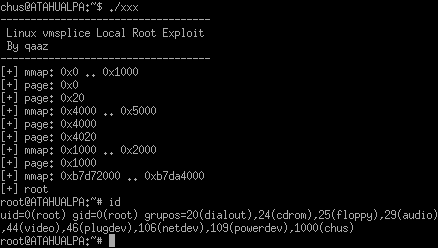
\includegraphics[height=.4\textheight]{L01/fot3.png}
\end{center}

\end{frame}

\begin{frame}
  \frametitle{Why Does Software Go Wrong?}

  \Large
  \begin{changemargin}{2em}
  5. Nonfunctional properties:
\begin{itemize}
  \item Leaks (yes, even in Java).
  \item Performance.
\end{itemize}
  \end{changemargin}

\end{frame}

\begin{frame}

  \frametitle{Why Does Software Go Wrong?}
  \begin{changemargin}{2em}

\Large
 Regressions to past bugs.
  \end{changemargin}
\end{frame}

\begin{frame}
  \frametitle{Avoiding Software Failures}

  \Large
    \begin{changemargin}{2em}
  \begin{itemize}
   \item test the software (in-house, externally)
   \item require validation suites for plugins
   \item code review
   \item better design (``write better code!'')
   \item include fewer features
   \item defensive programming \\~~~(especially for plugins)
  \end{itemize}
    \end{changemargin}
  
\end{frame}

\begin{frame}
  \frametitle{Mitigation: Failure is Inevitable}

  \Large
  \begin{changemargin}{2em}
  Software never completely works.\\[1em]

  Aim: make software that is good enough.
  \end{changemargin}

\end{frame}

\begin{frame}
  \frametitle{Coping with an Imperfect World}

    \begin{changemargin}{2em}
{\Large
  \begin{itemize}
   \item disclaim liability
  \end{itemize}
}
\begin{quote}
25. LIMITATION ON AND EXCLUSION OF DAMAGES. You can recover from
Microsoft and its suppliers only direct damages up to the amount you
paid for the software. You cannot recover any other damages, including
consequential, lost profits, special, indirect or incidental damages.
\end{quote}
\hfill (Vista license)
    \end{changemargin}
    
\end{frame}

\begin{frame}
  \frametitle{Coping with an Imperfect World}

  \Large
  \begin{changemargin}{2em}
  
  \begin{itemize}
   \item disclaim liability
   \item release patches
   \item backup/replicate user data
   \item defensive programming
  \end{itemize}
  \end{changemargin}
\end{frame}

\begin{frame}
  \frametitle{Ways of Testing Software}

  \Large
    \begin{changemargin}{2em}

  \begin{itemize}
   \item compile it
   \item<2-> run it on one input 
   \item<3-> run it on many inputs
   \item<4-> run it on a representative set of inputs
   \item<5-> run it on all inputs (static analysis)
  \end{itemize}
    \end{changemargin}

\end{frame}

\begin{frame}
  \frametitle{Other Testing Concerns}

  \begin{changemargin}{2em}
\Large
  \begin{itemize}
  \item Integration testing
  \item Nonfunctional properties
  \item Regression tests
  \end{itemize}
  \end{changemargin}
\end{frame}

\part{About This Course}
\begin{frame}
  \partpage
\end{frame}

\begin{frame}

  \frametitle{Goals of This Course}

    \begin{changemargin}{2em}

  \begin{itemize}

  \item You will be able to create and evaluate test suites for reasonably-sized
software systems.\\[1em]

  \item You will learn how to use and write tools for software maintenance and
verification (particularly automated testing tools).\\[1em]

  \end{itemize}
    \end{changemargin}

\end{frame}


\begin{frame}
\frametitle{Part I: Defining Test Suites}
\begin{changemargin}{2em}
\Large
Key questions:\\
\begin{itemize}
\item find interesting inputs;
\item know when to stop looking.
\end{itemize}
\end{changemargin}
\end{frame}

\begin{frame}
\frametitle{Generating Test Suites}
\begin{changemargin}{2em}
\Large
We'll see:
\begin{itemize}
\item open-ended exploratory testing;
\item statement/branch coverage;
\item graph-based models of program state; integrating design documentation;
\item automatically generating inputs: grammars, fuzzing.
\end{itemize}~\\[-1em]
\end{changemargin}
\end{frame}

\begin{frame}
\frametitle{Evaluating Test Suites}
\begin{changemargin}{2em}
\Large
How good is your test suite?
\begin{itemize}
\item coverage
\item mutation
\end{itemize}
\end{changemargin}
\end{frame}

\begin{frame}
\frametitle{Part II: Engineering Test Suites}
\Large
\begin{changemargin}{2em}
What are best (and worst) practices for implementing test suites?
\begin{itemize}
\item xUnit
\item web-based testing
\item mock objects
\item refactoring tests
\item refactoring code to be testable
\item continuous integration
\item flaky tests
\end{itemize}
\end{changemargin}
\end{frame}

\begin{frame}
\frametitle{Part III: Tools for Verification \& Validation}
\Large
\begin{changemargin}{2em}
What's out there beyond testing?
\begin{itemize}
\item concept: static vs. dynamic analysis
\item static approaches
\item dynamic approaches
\item human-based approaches: code review, bug reporting
\end{itemize}
\end{changemargin}
\end{frame}

\begin{frame}
\frametitle{Bonus: Debugging and the Scientific Method}
\Large
\begin{changemargin}{2em}
Don't: randomly debug your code.\\[1em]
Do: Make hypotheses and verify them.\\[2em]

Reference: Andreas Zeller. \emph{Why Programs Fail: a Guide to Systematic Debugging.}
\end{changemargin}
\end{frame}

\part{Defining some terms}
\begin{frame}
 
  \partpage
\end{frame}


\begin{frame}

  \frametitle{Terminology}
  
  \begin{changemargin}{2em}
\Large
\alert{Validation}: evaluating software prior to release to 
ensure compliance with intended usage.\\[1em]

\alert{Verification}: determining whether products of a given phase
of the development process fulfill requirements established in a 
previous phase.
  \end{changemargin}

\end{frame}

\begin{frame}

\frametitle{Terminology}
\Large

  \begin{changemargin}{2em}
\alert{Software fault}: static defect in the software.\\[1em]

\alert{Software error}: incorrect internal state that is the manifestation
of some fault.\\[1em]

\alert{Software failure}: External, incorrect behaviour \\ 
\hspace*{2em} (as in ``epic fail'').
  \end{changemargin}

\end{frame}

\begin{frame}

\frametitle{Testing vs. debugging}
\Large
  \begin{changemargin}{1em}

\alert{Testing}: \\
\hspace*{1em} evaluating software by observing its execution.\\[1em]

\alert{Debugging}: \\
\hspace*{1em} finding (and fixing) a fault given a failure.
  \end{changemargin}

\end{frame}

\begin{frame}
\Large
\frametitle{Problems with Manual Testing}

  \begin{changemargin}{2em}

\begin{itemize}
\item Testing tasks are often repetitive\\ (i.e. boring).
\item It is easy to make mistakes while carrying out tests.
\end{itemize}
  \end{changemargin}
\end{frame}

\begin{frame}
\frametitle{Automation}

  \begin{changemargin}{2em}
\Large
\alert{Automation} is key to successful testing:

\begin{itemize}
\item Enables you to run more tests more quickly.
\item Helps ensure coverage.
\end{itemize}
Designing test suites is real engineering\\ ~~~(in the broad sense).

  \end{changemargin}
\end{frame}

\end{document}
